%%%%%%%% ICML 2021 EXAMPLE LATEX SUBMISSION FILE %%%%%%%%%%%%%%%%%
\documentclass{article}
\usepackage[]{algorithm2e}
\usepackage{algorithmic}
\usepackage{algorithm}
% Recommended, but optional, packages for hs and better typesetting:
\usepackage{microtype}
\usepackage{graphicx}
\usepackage{amsmath}
\usepackage{amsfonts}
\usepackage{appendix}
\usepackage{subfigure}
\usepackage{booktabs} % for professional tables
\usepackage{hyperref}
% Attempt to make hyperref and algorithmic work together better:
\newcommand{\theHalgorithm}{\arabic{algorithm}}
\usepackage{icml2021}
\usepackage{float}
\usepackage{enumitem}

\begin{document}
\twocolumn[
\icmltitle{Reinforcement Learning 2024
Assignment 3: Policy-based Reinforcement Learning}

\icmlsetsymbol{equal}{*}
\begin{icmlauthorlist}
\icmlauthor{Sherry Usman}{equal,to}
\icmlauthor{Qin Zhipei}{equal,to}
\icmlauthor{Megan Mirnalini Sundaram R}{equal, to}
\end{icmlauthorlist}

\icmlaffiliation{to}{Leiden University}

% You may provide any keywords that you
% find helpful for describing your paper; these are used to populate
% the "keywords" metadata in the PDF but will not be shown in the document
\icmlkeywords{Machine Learning, Deep Q-Learning, Experience Replay, Target Network}

\vskip 0.3in
]

\begin{abstract}

\end{abstract}

\section {Introduction}
In this paper we will delve into the Lunar Lander environment taken from the OpenAI Gym library. The Lunar Lander game is a classical reinforcement learning environment where the goal is to optimise the trajectory of a rocket such that it lands between the two flags.
 While a number of different techniques can be used to solve this problem, our paper specifically concentrates on the use of  \textbf{REINFORCE} and \textbf{Actor-Critic}. Through this paper, we hope to provide the specifications of various Policy Gradient methods while also including the tried and tested hyper-parameters that produce the best results.%$$ best exploration-to-exploitation ratio. \newline

\begin{figure}[htbp]
\centering
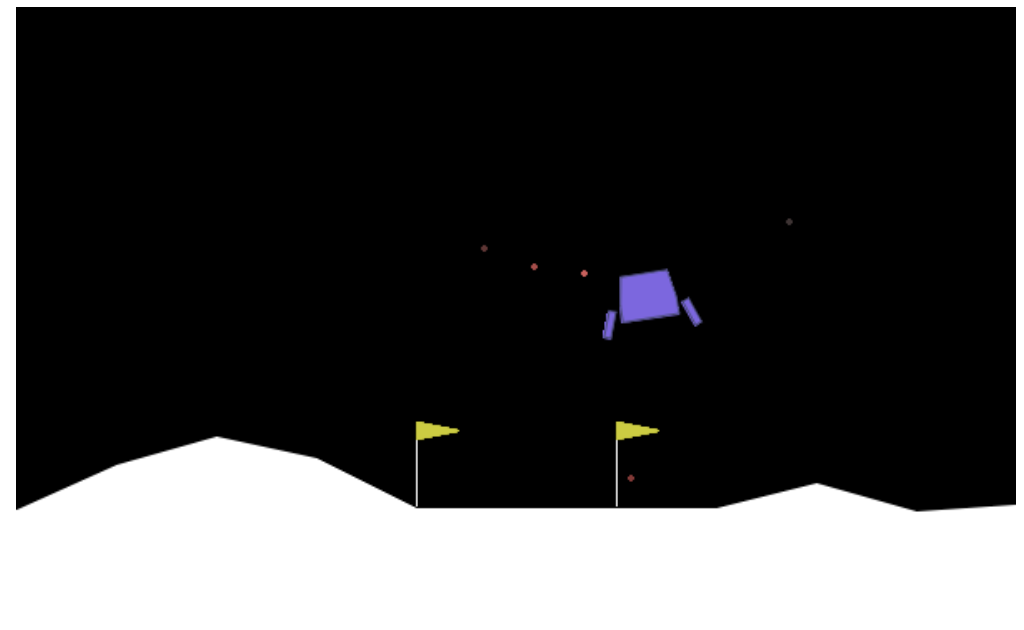
\includegraphics[width=0.7\linewidth]{Report/images/visualisation.png}
\caption{\label{fig:Visualization of the Cart-pole} A visualisation of the Lunar Lander problem}
\end{figure}

%\label{Introduction and General Strategy}

The Lunar Lander environment poses a number of unique challenges compared to the environments we have encountered previously. As shown in \emph{Table 1}, While the action space $A$ is still discrete with four potential actions, the observation space is an 8-dimensional vector, the positional coordinates of the lunar lander (x and y), its linear velocities in x and in y respectively, its angle, its angular velocities and two boolean values that represent whether each leg is in contact with the ground or not. The inclusion of a continuous action or state space makes tabular/value-based reinforcement learning algorithms quickly unfeasible as the cost of storing the values for each state-action pair makes our problem much more complex. \newline
Thus, to tackle this problem we use Policy Gradient methods which can handle continuous state and action spaces much better as they directly optimise the expected return and can output continuous action distributions, making them also suitable for continuous action spaces. Furthermore, since Policy Gradient methods do not need state-action pairs to approximate values they do not run the risk of getting stuck in local optima like value-based methods and can approximate complex non-linear relationships more accurately than value-based algorithms.

\begin{table}[htbp]
\centering
\begin{tabular}{|l|c|}
\hline
\textbf{Value} & \textbf{Action} \\
\hline
0  & Do nothing \\
\hline
1 & fire left orientation engine \\
\hline
2  & fire main engine \\
\hline
3 & fire right orientation engine  \\
\hline
\end{tabular}
\caption{Action Space of Lunar Lander Environment}
\label{tab:hyper-parameters}
\end{table}



\section{Framework}
For our implementation of Policy Gradient Methods, we used the Python \textbf{Pytorch} package. Our initial structure is as follows: an input layer of size 8 corresponding to the size of the observation space. This input layer feeds into a first hidden layer with 128 nodes. This then feeds into a hidden layer comprising of 128 nodes which finally outputs to a layer comprising of 1 node representing the action that should be taken. Since the Lunar Lander environment is also highly stochastic and affected by noise, to reduce noise in our graphs we computed different algorithms over 1000 episodes and averaged the results every 5 episodes to capture the general trends. Furthermore, we are aware that total rewards is not always the best parameter to measure algorithm accuracy as the number of timesteps in each episode may differ and lead to exploding or shrinking rewards. Thus, in some cases we also include another parameter to measure accuracy which is the number of timesteps.

%In this section we experiment with various hyper-parameters such as batch size, learning rates and more while also fine-tuning our neural network by modifying the number of hidden layers and neurons in each layer.% Since this environment is also highly stochastic, we de-noise by testing over 1000 episodes and averaging our results over every 10 episodes.
%For 

\section{Policy-Based Reinforcement Learning}
The policies we looked at in the previous papers were \emph{value-based}. This means that they looked at state-value pairs in the environment and approximated the rewards of such pairs using different exploration strategies like Boltzmann or Epsilon-Greedy. Policy based reinforcement learning methods differ from value-based method as they do not utilize a value function to determine the next possible action. Used primarily in  continuous action space RL environments, policy based reinforcement learning methods use a parameterized policy function $\pi_\theta$ where $\theta$ represents the parameters of the function.
\par During training the agent iteratively interacts with the environment over multiple episodes. After a number of episodes the collected data known as the trajectory $\tau$ is evaluated to understand the performance of the policy. If $\tau$ yields high rewards then the parameters $\theta$ are adjusted in such a way that the likelihood of taking actions similar to the actions in this trajectory is increased. On the other hand if the trajectory $\tau$ yields lower rewards then the parameters $\theta$ are adjusted in such a way that the likelihood of taking actions similar to such actions is decreased. This process of iteratively evaluating the trajectories and updating the parameters according to the obtained rewards/losses helps to refine the policy to maximize cumulative rewards in the long run \cite{plaat-deeprl}. 
\par
There are a number of different policy-based reinforcement learning algorithms. However for this paper, we are limiting the scope of our research to the algorithms listed below: 

\begin{itemize}[itemsep=0pt]
\item REINFORCE
\item Actor-Critic
\item Actor-Critic with Bootstrapping
\item Actor-Critic with Baseline Subtraction
\item Actor Critic with Bootstrapping and Baseline Subtraction
\end{itemize}
These algorithms are discussed in the future sections. 

\par For any reinforcement learning algorithm it is necessary to decide on an action selection policy. Traditional action selection algorithms used before such as Boltzmann or E-greedy cannot be used in this paper as they are better suited for value-based reinforcement learning algorithms working with a discrete action space and/or state space. This is because both epsilon-greedy and Boltzman are algorithms that scans potential actions that can be taken by the agent at a particular state and calculates their value, which helps inform the agent's next step. This is not possible in Policy Gradient methods which are less concerned with state-action pairs and more with the policy function. 
\par Thus in this paper we work with \textbf{Entropy Regularisation}. Entropy regularisation is an exploration technique that helps balance the exploration to exploitation ratio by encouraging the agent to explore more diverse actions and unfamiliar spaces. It does this by increasing by adding an entropy term to the loss function to promote action diversity and preventing sub-optimising to local rewards. The entropy term is defined in the equation below. %

\begin{equation*}
H(X) = - \sum \pi(x) log(\pi(x)) %t + 1] 
\end{equation*}
where
\begin{itemize}
\renewcommand\labelitemi{.}
\item x is the set of possible actions
\item $\pi(x)$ is a function representing the probability of taking an action x
\item H(X) is the entropy of the action distribution capturing the randomness of taking an action x
\end{itemize}
\subsection{REINFORCE}
\par REINFORCE is a commonly used Policy-based Reinforcement Learning algorithm which is also termed as a classic Monte-Carlo Policy Gradient algorithm. It was first introduced in 1992 by Ronald J. Williams with an aim to maximise expected cumulative rewards by adjusting the policy parameters. It does this by learning from the agent trajectory (including the visited states, executed actions and incurred rewards) and estimating gradients. Because it needs a full trajectory in order to construct a sample space it is updated as an off-policy algorithm. 
\begin{equation}
\pi_\theta(a, s) = Pr(A_t = a | St = s, \theta_t = \theta)
\end{equation}
The equation above helps us recall the policy function $\pi_{\theta}(a, s)$ which indicates the probability of taking an action a in the state s with the parameters $\theta$.
We can also define a trajectory $\tau$ as the sum of rewards when following a particular path. This is shown in the equation below.
\begin{equation}
R(\tau) = [\sum_{t=0}^{T-1}r_t] 
\end{equation}

\par The REINFORCE algorithm optimises the policy function $\pi_{\theta}(a,s)$ by fine-tuning its parameters $\theta$ such that it increases the likelihood of actions in trajectories $\tau$ which lead to higher cumulative rewards. It does this by calculating the total expected rewards J($\theta$) with respect to a particular parameter value $\theta$ and adjusting $\theta$ accordingly. Thus, J($\theta$) is optimised as shown in equation 2.
\begin{equation}
\nabla J(\theta) = E_{\pi_\theta}[ R(\tau)] =   E_{\pi_\theta} (\sum_{t=0}^{T-1} \nabla log\pi_\theta(a_t s_t) R(\tau)]
\end{equation}

where $\nabla J(\theta)$ represents the gradient in the expected return function J($\theta$), E$\pi_\theta$ denotes the expectation over trajectories R sampled under policy $\pi_\theta$, $R_{\tau}$ indicates the rewards obtained from the trajectory $\tau$ and $\pi_\theta$ indicates the policy function with parameters $\theta$.  \newline
%Thus $\theta$ is optimised to be equal to the gradient ascent of the partial derivative with respect to $\theta$ of $J(\theta)$. The equation for optimisation is shown below.
%\begin{equation}
%\theta = \theta + \frac{\mathrm{d}  }{\mathrm{d} \theta} J(\theta)
%\end{equation}
%Based on this, the expected cumulative rewards is updated.

The algorithm for REINFORCE can thus be defined as follows. 
\begin{algorithm}[htbp]
\caption{REINFORCE Algorithm}
\SetAlgoLined
\DontPrintSemicolon
\small % Set font size to small
\KwData{parameter $\theta$, policy function $\pi_\theta$, maximum timesteps $T$, number of episodes $E$, learning_rate $\alpha$ }
\KwResult{Selected action}
Initialise $\theta$ arbitrarily\;\\
\For{$e = 1$ \KwTo $E$}{
    Initialise state $s$\;
    \For{$t = 1$ \KwTo $T-1$}
    {
     \item Sample action $a$ from $\pi_\theta$\;
     \item Execute action $a$ and get the next state $s_{t+1}$ and  reward $r_t$\; 
     \item $\theta \leftarrow \theta + \alpha \cdot \nabla_\theta \log \pi_\theta(a_t | s_t) R(\tau)$;
    }
}
Return parameter $\theta$
\end{algorithm}

The results of REINFORCE without entropy regularisation can be seen below.

\begin{figure}[htbp]
\centering
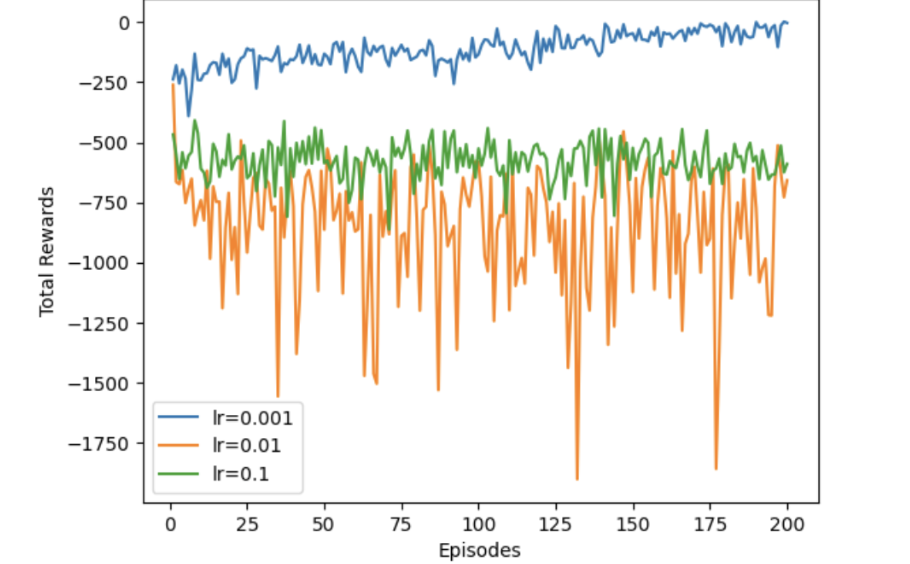
\includegraphics[width=0.9\linewidth]{Report/images/reinforce_basic_image1.png}
\caption{\label{fig:Reinforce Rewards}The figure above shows the rewards of REINFORCE without entropy regularisation with different learning rates. As we can see, almost learning rates show a rising trend of rewards, with the graph for learning rates 0.01 and 0.001 showing the most promise. }
\end{figure}


\begin{figure}[htbp]
\centering
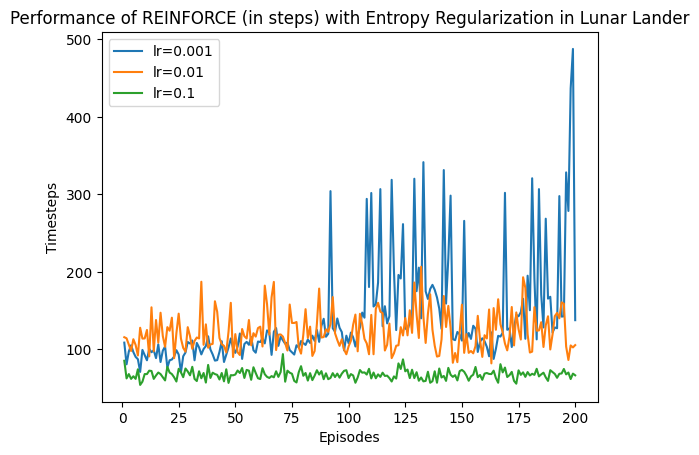
\includegraphics[width=0.9\linewidth]{Report/images/reinforce_basic_image2.png}
\caption{\label{fig:ReinforceEntropy_Rewards}The figure above shows the steps of REINFORCE without entropy regularisation with different learning rates. As we can see, almost learning rates show a rising trend of steps, with the graph for learning rates 0.01 and 0.001 showing the most promise. }
\end{figure}


Figure 2 and 3 shows our results for REINFORCE without entropy regularisation. While REINFORCE is touted as a simpler Policy Gradient method it can often suffer from high variances causing slower convergence to optimal values. This is very visible from the results. Even after an average results over 1000 episodes, we are unable to see a dramatic rise in learning as we were hoping. However, we can see the effect of learning rate on model performance as learning rates of 0.001 and 0.01 outperform learning rate of 0.1. To improve our existing results we decided to implement a version of REINFORCE that includes entropy regularisation and as seen from our figure 4, there is much better learning and faster convergence as learning rates begin rising. This is because the inclusion of an entropy term to the loss function helps penalise trajectories with lesser randomness (or entropy) and thus encourages the policy network to explore more diverse state and action spaces, increasing exploration and preventing getting stuck in suboptimal local maxima. 

\begin{figure}[htbp]
\centering
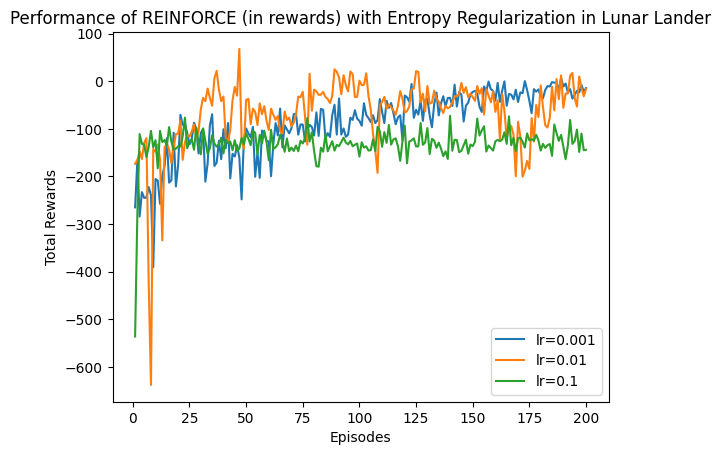
\includegraphics[width=0.9\linewidth]{Report/images/entropy_regularisation.png}
\caption{\label{fig:ReinforceEntropy_Rewards_LR}The figure above shows the rewards of REINFORCE with entropy regularisation with different learning rates. As we can see, all learning rates show a rising trend of rewards, with the graph for learning rates 0.01 and 0.001 showing the most improvement and the learning rate 0.1 stabilising but not showing much improvement. }
\end{figure}


\begin{figure}[htbp]
\centering
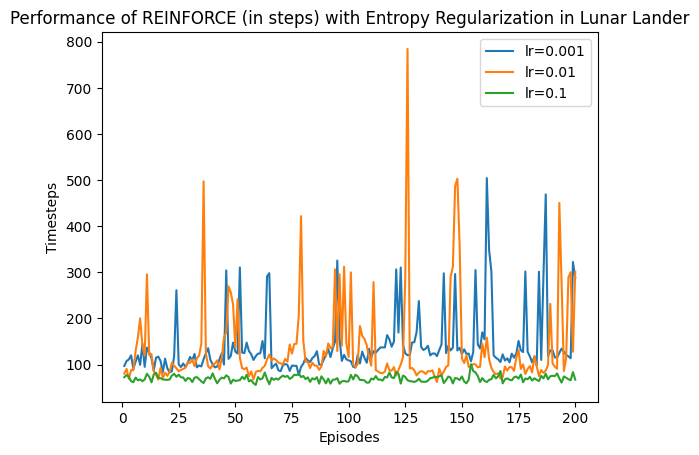
\includegraphics[width=0.9\linewidth]{Report/images/entropy_regularisation_2.png}
\caption{\label{fig:ReinforceEntropy_Rewards_Steps}The figure above shows the total steps of REINFORCE with entropy regularisation with different learning rates. As we can see, all learning rates show a rising trend of rewards, with the graph for learning rates 0.01 and 0.001 showing the most improvement and the learning rate 0.1 stabilising but not showing much improvement. }
\end{figure}

  

\subsection{Actor-Critic Methods}
Actor Critic methods are Temporal Difference methods and have a separate memory structure to store the policy function independent of the value function. They generally have two neural networks: a policy structure known as an \emph{actor} and an estimated value function known as the \emph{critic}. While the policy function (or actor) returns a probability distribution of actions that can be taken in specific states, a value function (or the critic) determines the expected reward gained by following the policy. Thus the value function is called a critic as it criticises the actions taken by the actor in the form of a TD error. This scalar signal indicates whether the actions taken by the agent are better or worse than what the critic expected. 
\par The TD error can be evaluated as follows in the following equation
\begin{equation*}
\delta_{t} = R_{t+1} + \gamma * V_t(S_{t+1})-V_t(S_t)
\end{equation*}
 where 
\begin{itemize}[itemsep=0pt]
\renewcommand\labelitemi{.}
\item $\delta_{t}$ is the temporal difference error at timestep $t$
\item $R_{t+1}$ is the reward for transitioning from state $S_t$ to the state $S_{t+1}$
\item $\gamma$ is the discount factor which discounts future rewards
\item $V_t(S_{t+1})$ is the estimated value of going to state $S_{t+1}$ at timestep t according to the critic. This represents the estimated cumulative rewards that can be gained from step $S_{t+1}$ onwards.
\item $V_t(S_t)$ is the estimated value of going to state $S_t$ according to the critic. This represents the estimated total rewards that can be gained from step $S_{t}$ onwards.
\end{itemize}
Thus, a positive TD error ($\delta_{t}$ \textgreater 0) indicates that the value of transitioning from state $S_t$ to $S_{t+1}$ is greater than expected and thus the action responsible should be taken more often. On the other hand a negative TD error ($\delta_{t}$ \textless 0) indicates that the value of transitioning from state $S_t$ to $S_{t+1}$ is lesser than expected and thus the action responsible should be avoided in the future. Thus, through this iterative process of updating the TD error the Actor Critic algorithm tends to strike a balance between exploration and exploitation. The actor explores the state space and taking more diverse actions and the critic evaluating the consequences of the actions. When the actions are more risky and produce lesser expected returns the TD error is negative and when they are more fruitful and produce higher expected returns the TD error is positive.


% \newline
%\newline As used in REINFORCE, the policy gradient is given by 
%\newline 
%\begin{equation*}
%\nabla_\theta J(\theta) = \mathbb{E}_\pi[\sum _{t=0}^{T-1} \nabla_\theta log\pi_\theta (a_t|s_t)G_t]
%\end{equation*}
%\begin{figure}[htbp]
%\centering
In the REINFORCE algorithm, because the entire episode must be sampled, its variance is high. The Actor Critic method combines value-based and policy-based methods, achieving both low variance and low bias. The Actor Critic method incorporates the bootstrapping technique to improve estimates of cumulative rewards. By using bootstrapping, the Actor Critic method can use the Critic's immediate feedback to adjust the Actor's strategy, thus achieving a better balance between exploring the environment and learning optimized action strategies.


\subsubsection{Bootstrapping}
\par A variation of Actor-Critic incorporates a boot-strapping technique.  In the REINFORCE algorithm, because the entire episode must be sampled, its variance is high. The Actor Critic method combines value-based and policy-based methods, achieving both low variance and low bias. The Actor Critic method incorporates the bootstrapping technique to improve estimates of cumulative rewards. By using bootstrapping, the Actor Critic method can use the Critic's immediate feedback to adjust the Actor's strategy, thus achieving a better balance between exploring the environment and learning optimized action strategies.
\par Similar to the traditional actor critic method, there is an actor who learns the policy and there is a critic which criticises/evaluates the rewards gained from following the policy (the value of particular state-action pairs Q(s,a)) . However, in the case of Actor Critic with bootstrapping, the critic uses bootstrapping to update the value Q of the state-action pairs, harking back to value-based methods. 

The algorithm for Actor-Critic with Bootstrapping is given below \cite{plaat-deeprl}
\begin{algorithm}[htbp]
\caption{Actor-Critic with Bootstrapping}
\SetAlgoLined
\DontPrintSemicolon
\small % Set font size to small
\KwData{parameter $\theta$, policy function $\pi_\theta$, maximum timesteps $T$, number of episodes $E$, estimation depth $n$, learning rate $\alpha$, value function $V_\phi (s)$}
\KwResult{Selected action}
Initialise $\theta$ and $\phi$ arbitrarily\;\\
\For{$e \in 1$ \KwTo $E$}
{
    \item Initialise state $s$\;
    \item Sample trajectory $\tau$ = ${s_0,a_0,r_1,....,s_T}$ for $\pi_\theta(a|s)$
     \item 
    \For{$t = 1$ \KwTo $T-1$}
    {
     \item Compute cumulative reward $\hat{Q}_n(s_t,a_t)$ for the n-step target
     \newline \(\hat{Q}^(s_t,a_t) = \sum_{k=0}^{n-1}\gamma^k\cdot r_{t+k} + \gamma_n \cdot V_\phi (s_{t+n})\)
    }
    \item Compute descent advantage loss $\phi$
    \item Compute ascent policy gradient $\theta$
}
\State \Return parameter $\theta$
\end{algorithm}

\begin{figure}[htbp]
    \centering
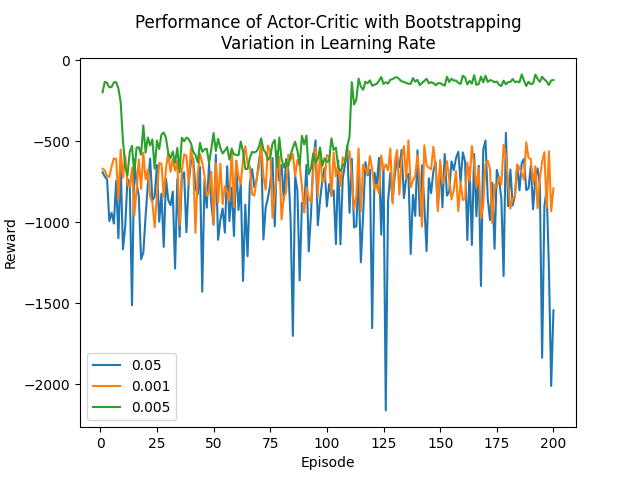
\includegraphics[width=0.9\linewidth]{Report/images/Performance_of_Actor_Critic_BS_LR.png}
\caption{\label{fig:ActorCritic for different learning rates}The figure above shows the result of Actor Critic with different learning rates. As we can see, all learning rates show a rising trend of rewards, with the graph for learning rate 0.01 showing the most improvement}
\end{figure}

\begin{figure}[htbp]
\centering
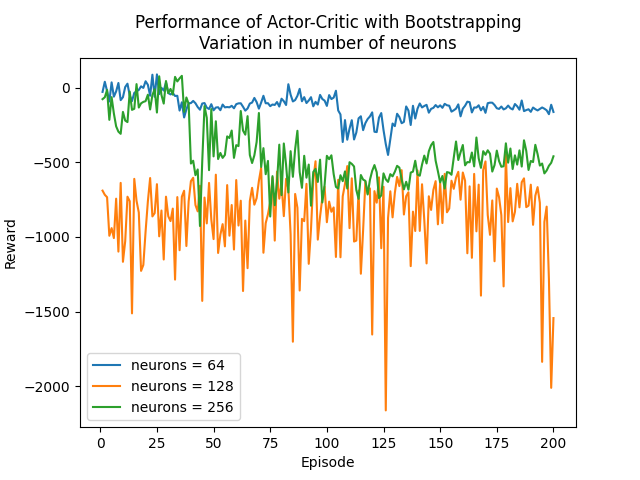
\includegraphics[width=0.9\linewidth]{Report/images/Performance_of_Actor_Critic_BS_Neurons.png}
\caption{\label{fig:ActorCritic for different Neurons}The figure above shows the result of Actor Critic with different neurons. }
\end{figure}


\begin{figure}[htbp]
\centering
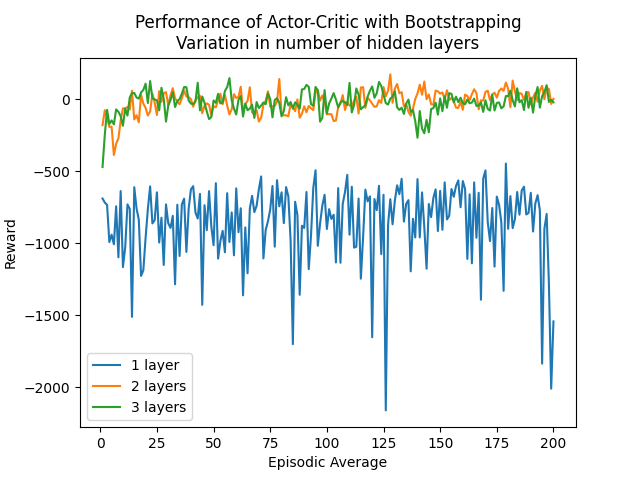
\includegraphics[width=0.9\linewidth]{Report/images/Performance_of_Actor_Critic_BS_Layers.png}
\caption{\label{fig:ActorCritic for different Hidden Layers}The figure above shows the result of Actor Critic with different hidden layers}
\end{figure}




\subsubsection{Baseline Subtraction}
Actor-Critic algorithms could also employ baseline subtraction which is a technique used to reduce the variance by using a baseline. We recall the previous policy gradient function denoted by 
\begin{equation*}
\nabla_\theta J(\theta) = \mathbb{E}_\pi[\sum _{t=0}^{T-1}  \nabla_\theta \log\pi_\theta (a_t|s_t)G_t]
\end{equation*}
By subtracting a baseline $b(s_t)$ from the cumulative reward helps reduce make them smaller and more stable, reducing variance. The updated policy gradient function after baseline subtraction is shown below. 
\begin{equation*}
\nabla_\theta J(\theta) = \mathbb{E}_\pi[\sum _{t=0}^{T-1}  \nabla_\theta\log\pi_\theta (a_t|s_t)G_t - b(s_t)]
\end{equation*}
\begin{algorithm}[htbp]
\caption{Actor-Critic with Baseline Subtraction}
\SetAlgoLined
\DontPrintSemicolon
\small % Set font size to small
\KwData{parameter $\theta$, policy function $\pi_\theta$, maximum timesteps $T$, number of episodes $E$, estimation depth $n$, learning rate $\alpha$, value function $V_\phi (s)$}
\KwResult{Selected action}
Initialise $\theta$ and $\phi$ arbitrarily\;\\
\For{$e = 1$ \KwTo $E$}
{
    Initialise state $s$\;
     \item Sample trajectory $\tau$ for $\pi_\theta$
     \item
    \For{$t = 1$ \KwTo $T-1$}
    {
     \item Compute advantage function using the cumulative reward and the value function;
     \(\hat{A}_n(s_t,a_t) = \hat{Q}_n(s_t,a_t) - V_\phi(s_t)\)
    }
    \item Compute descent advantage loss $\phi$
    \item Compute ascent policy gradient $\theta$
}
\State \Return parameter $\theta$
\end{algorithm}
\subsubsection{Bootstrapping and Baseline Subtraction}
Actor-Critic algorithms combine both Bootstrapping and Baseline Subtraction
\par Descent Advantage Loss is calculated as
\begin{equation*}
\phi \leftarrow \phi - \alpha * \nabla_\phi\Sigma_t(\hat{A}_n(s_t,a_t))^2
\end{equation*}
Ascent Policy Gradient is calculated as
\begin{equation*}
\theta \leftarrow \theta + \alpha * \Sigma_t[\hat{A}_n(s_t,a_t)*\nabla_\theta\log\pi_\theta(a_t|s_t)]
\end{equation*}
\begin{algorithm}[htbp]
\caption{Actor-Critic with Bootstrapping and Baseline Subtraction}
\SetAlgoLined
\DontPrintSemicolon
\small % Set font size to small
\KwData{parameter $\theta$, policy function $\pi_\theta$, maximum timesteps $T$, number of episodes $E$, estimation depth $n$, learning rate $\alpha$, value function $V_\phi (s)$}
\KwResult{Selected action}
Initialise $\theta$ and $\phi$ arbitrarily\;\\
\For{$e = 1$ \KwTo $E$}
{
    Initialise state $s$\;
     \item Sample trajectory $\tau$ for $\pi_\theta$
     \item
    \For{$t = 1$ \KwTo $T-1$}
    {
     \item Compute cumulative reward $\hat{Q}_n(s_t,a_t)$  for the n-step target
     \item Compute advantage function using the cumulative reward and the value function;
     \(\hat{A}_n(s_t,a_t) = \hat{Q}_n(s_t,a_t) - V_\phi(s_t)\)
    }
    \item Compute descent advantage loss $\phi$
    \item Compute ascent policy gradient $\theta$
}
\State \Return parameter $\theta$
\end{algorithm}
\begin{figure}[htbp]
\centering
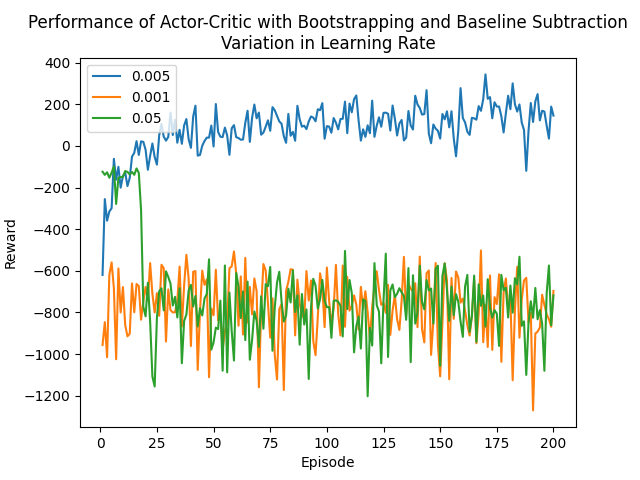
\includegraphics[width=0.9\linewidth]{Report/images/Performance_of_Actor_Critic_BSandBS_LR.png}
\caption{\label{fig:ActorCriticBS2-different learning rates}The figure above shows the result of Actor Critic with different learning rates. As we can see, all learning rates show a rising trend of rewards, with the graph for learning rate 0.01 showing the most improvement}
\end{figure}

\begin{figure}[htbp]
\centering
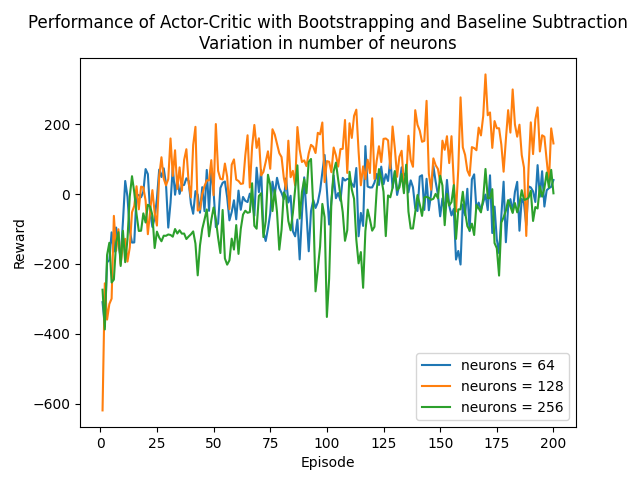
\includegraphics[width=0.9\linewidth]{Report/images/Performance_of_Actor_Critic_BSandBS_Neurons.png}
\caption{\label{fig:ActorCriticBS2-different neurons}The figure above shows the result of Actor Critic with different number of neurons}
\end{figure}

\begin{figure}[htbp]
\centering
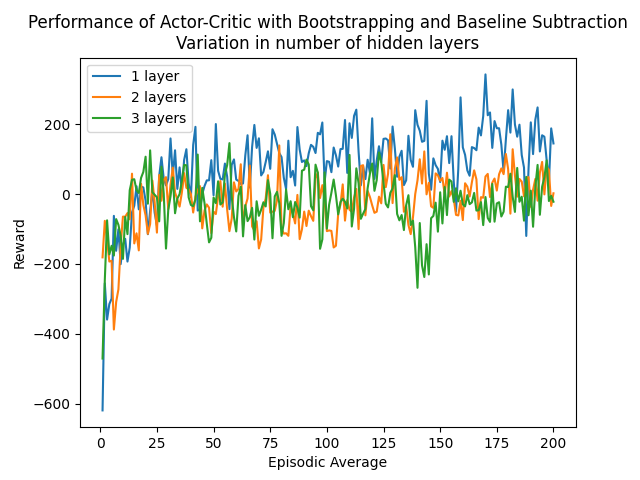
\includegraphics[width=0.9\linewidth]{Report/images/Performance_of_Actor_Critic_BSandBS_Layers.png}
\caption{\label{fig:ActorCriticBS2-different hidden layers}The figure above shows the result of Actor Critic with different hidden layers}
\end{figure}


\section{Goals Achieved}
\subsection{Effects of policy gradients on variance}
\subsection{Effects of bootstrapping on the policy gradients}
\subsection{Comparison of Performance}
\subsection{Effect of entropy regularization on performance}

\bibliography{Report/references}
\bibliographystyle{Report/reference_style}
\end{document}

